\documentclass[a4paper,11pt]{article}

\usepackage[utf8x]{inputenc}
\SetUnicodeOption{mathletters}
\SetUnicodeOption{autogenerated}

\usepackage[italian]{babel}
\usepackage{booktabs}
\usepackage{mathpazo}
\usepackage{graphicx}
\usepackage[left=2cm, right=2cm, bottom=3cm]{geometry}
\frenchspacing

\begin{document}
\noindent {\Large Olimpiadi di Informatica: selezioni nazionali 2012}
\vspace{0.5cm}

\noindent {\Huge Disegna senza sollevare la matita (\texttt{matita})}


\section*{Descrizione del problema}
   
Sai risolvere il classico puzzle di disegnare una casetta (con una X
nel suo riquadro centrale) senza mai sollevare la
matita dal foglio? 

\begin{figure}[h!]
  \centering
  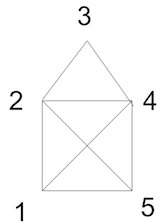
\includegraphics{casetta.png}
  \caption{Disegna questa casetta senza mai sollevare la
matita dal foglio.}
\end{figure}

In generale, sono dati $N$ vertici, numerati da $1$ a
$N$, e $M$ lati che li collegano. Sapresti indicare in quale sequenza attraversare i lati, e per ciascuno di essi in quale direzione, in modo che il vertice cui ci conduce ciascun lato coincida col vertice da cui ci preleva il lato successivo (senza alzare quindi la matita)? La sfida è di riuscire ad attraversare ciascun lato una ed una volta sola.
Ti è possibile riuscire a farlo tornando infine al vertice di partenza?

\section*{Input}
Si legga l'input da `stdin`.
La prima riga contiene $T$, il numero di testcase (istanze) da risolvere. Seguono $T$
istanze del problema. Per ogni istanza, la prima riga contiene quattro numeri interi $N$,
$M$, $A$ e $B$ separati da uno spazio:
il numero di vertici, il numero di lati che si richiede di attraversare (ogni lato una ed una volta sola, dovrai decidere tu in quale direzione), il vertice di
partenza, e quello di arrivo.
Le successive $M$ righe offrono, uno per riga, gli $M$ lati del puzzle, ciascun rappresentato da una
coppia non-ordinata di interi nell'intervallo $[1,N]$, separati da uno spazio (questi interi sono i nomi dei vertici collegati dal lato in questione). Per ciascun lato "$X$ $Y$" dovrai scegliere se attraversarlo da $X$ ad $Y$ oppure da $Y$ ad $X$, oltre che stabilire in quale ordine vadano attraversati i lati.

\section*{Output}  
Per ciascuna istanza, prima di poter leggere l'istanza successiva, occorre trasmettere su `stdout` l'output che sarà così strutturato:
per ogni riga dell'input intesa a rappresentare un lato del puzzle (ossia nel formato "$X$ $Y$"), l'output dovrà contenere una riga "$X$ $Y$" se il lato viene percorso da $X$ a $Y$, oppure una riga "$Y$ $X$" se il lato viene percorso da $Y$ a $X$.
Le righe in output saranno pertanto $M$, ma riordinate rispetto alle $M$ rispettive righe dell'input in modo da specificare inoltre in quale ordine gli $M$ lati dell'input vengano attraversati: per la prima di queste righe deve valere la condizione che $X = A$. Il vertice $X$ di ciascun altra riga deve coincidere col vertice $Y$ della riga precedente (non devi staccare mai la matita dal foglio), e per l'ultima riga deve valere anche che $Y=B$.


\section*{Esempi di input/output}

  
    \noindent
    \begin{tabular}{p{11cm}|p{5cm}}
    \toprule
    \textbf{File \texttt{input.txt}}
    & \textbf{File \texttt{output.txt}}
    \\
    \midrule
    \scriptsize
    \begin{verbatim}
1
5 8 1 5
1 4
2 3
5 4
2 1
2 4
3 4
1 5
5 2
\end{verbatim}
    &
    \scriptsize
    \begin{verbatim}
1 2
2 3
3 4
4 5
5 2
2 4
4 1
1 5
\end{verbatim}
    \\
    \bottomrule
    \end{tabular}
  
\section*{Note}
\begin{itemize}
  
    \item 
Viene garantito che sia sempre possibile disegnare senza alzare la matita. Nel caso vi siano più soluzioni valide, è sufficiente restituirne una qualsiasi.

    \item 
Nessun testcase presenta lati multipli che collegano la stessa coppia di vertici (se un lato di un'istanza è descritto dalla stringa "$X$ $Y$", nella stessa istanza non potrai ritrovare la stessa stringa e nemmeno la stringa "$Y$ $X$"). Inoltre non forniremo mai lati della forma "$X$ $X$". Tutti i vertici e tutti i lati devono essere attraversati dalla matita.

    \item 
    Per chi non lo avesse riconosciuto, questo è il noto problema affrontato dal matematico Eulero in un lavoro (1735) considerato l'atto di nascita della teoria dei grafi e della topologia.

\end{itemize}

% Subtasks
\section*{Subtask}

Il tempo limite per istanza (ossia per ciascun testcase) è sempre di $1$ secondo.

I testcase sono raggruppati nei seguenti subtask.

\begin{description}
  \item[\textbf{\hspace{1ex}[1 istanza] esempi\_testo:}] l'esempio del testo (disegna la casetta)
  \item [\textbf{[8 istanze] smallest:}] $N = 2, 3, 4$ ($M \leq 6$)
  \item [\textbf{[10 istanze] small:}] $N = 5, 6$ ($M \leq 12$)
  \item [\textbf{[30 istanze] medium:}] $N \leq 100$, $M \leq 500$
  \item [\textbf{[21 istanze] big:}] $N \leq 1\,000$, $M \leq 5\,000$
  \item [\textbf{[30 istanze] huge:}] $N \leq 10\,000$, $M \leq 50\,000$
\end{description}

In generale, quando si richiede la valutazione di un subtask vengono valutati anche i subtask che li precedono, ma si evita di avventurarsi in subtask successivi  fuori dalla portata del tuo programma che potrebbe andare in crash o comportare tempi lunghi per ottenere la valutazione completa della sottomissione. Ad esempio, chiamando:

\begin{verbatim}
    rtal -s wss://ta.di.univr.it/algo  connect -a size=medium  matita -- python my_solution.py
\end{verbatim}

\noindent
vengono valutati, nell'ordine, i subtask:\\

{\tt esempi\_testo}, {\tt smallest}, {\tt small}, {\tt medium}.\\

\noindent
Il valore di default per l'argomento {\tt size} è {\tt huge} che include tutti i testcase.\\


\end{document}
